\documentclass[conference]{IEEEtran}
\IEEEoverridecommandlockouts
% The preceding line is only needed to identify funding in the first footnote. If that is unneeded, please comment it out.
\usepackage{cite}
\usepackage{amsmath,amssymb,amsfonts}
\usepackage{algorithmic}
\usepackage{graphicx}
\usepackage{textcomp}
\usepackage{xcolor}
\usepackage[acronym]{glossaries}
\usepackage[english]{babel}
\usepackage[autolanguage]{numprint}
\usepackage{todonotes}
\usepackage{endnotes}
\usepackage{xcolor}
\usepackage{xspace}
\usepackage{numprint}


\renewcommand{\notesname}{Referenced URLs}
\newcommand{\citeurl}[1]{\endnote{{\scriptsize \url{#1}}}}

\newcommand{\toolname}[1]{{\scriptsize \texttt{#1}}}

\begin{document}

\title{Visualizing Git Repositories for Assessment in Software Engineering Education}
% \thanks{Identify applicable funding agency here. If none, delete this.}


\author{\IEEEauthorblockN{1\textsuperscript{st} Given Name Surname}
\IEEEauthorblockA{\textit{dept. name of organization (of Aff.)} \\
\textit{name of organization (of Aff.)}\\
City, Country \\
email address or ORCID}
\and
\IEEEauthorblockN{2\textsuperscript{nd} Given Name Surname}
\IEEEauthorblockA{\textit{dept. name of organization (of Aff.)} \\
\textit{name of organization (of Aff.)}\\
City, Country \\
email address or ORCID}
\and
\IEEEauthorblockN{3\textsuperscript{rd} Given Name Surname}
\IEEEauthorblockA{\textit{dept. name of organization (of Aff.)} \\
\textit{name of organization (of Aff.)}\\
City, Country \\
email address or ORCID}
\and
\IEEEauthorblockN{4\textsuperscript{th} Given Name Surname}
\IEEEauthorblockA{\textit{dept. name of organization (of Aff.)} \\
\textit{name of organization (of Aff.)}\\
City, Country \\
email address or ORCID}
\and
\IEEEauthorblockN{5\textsuperscript{th} Given Name Surname}
\IEEEauthorblockA{\textit{dept. name of organization (of Aff.)} \\
\textit{name of organization (of Aff.)}\\
City, Country \\
email address or ORCID}
\and
\IEEEauthorblockN{6\textsuperscript{th} Given Name Surname}
\IEEEauthorblockA{\textit{dept. name of organization (of Aff.)} \\
\textit{name of organization (of Aff.)}\\
City, Country \\
email address or ORCID}
}

\maketitle

\begin{abstract}
Practitioners apply various readily available tools to visualize version control system data (software repositories).
Since such tools target usually software engineering professionals but not educators, their potential benefits for assessment in software engineering education are not explored much.
In this paper we describe usage patterns of software repository visualizations, illustrate them on the tool prototype \toolname{git-truck}, 
% discuss challenges and opportunities of applying repository visualization for assessment in software engineering education.
and we discuss challenges for future tool builders.
\end{abstract}

\begin{IEEEkeywords}
\end{IEEEkeywords}

\section{Introduction}

\section{Related Work}

\section{Assumptions}

\section{The Tool Prototype: \toolname{git-truck}}

% The tool used in this case study is git-truck, v. 1.1.0. 
The tool \toolname{git-truck} is released under an open source license (MIT) and is available on Github\citeurl{https://github.com/git-truck/git-truck} and as Node package on the \toolname{npm} registry\citeurl{https://www.npmjs.com/package/git-truck}. 
It can be installed easily on any on which system \toolname{NodeJS} and the corresponding package manager \toolname{npm} are setup\citeurl{https://docs.npmjs.com/cli/v7/configuring-npm/install}.

Unlike many other software-as-a-service tools, \toolname{git-truck} is meant to be executed directly on personal computers.
That allows educators to assess also private or institutional repositories, which are usually not shared publicly via software forges like Github, Gitlab, Bitbucket, etc.

To assess a local \toolname{git} repository, the tool can be executed directly in a directory containing a repository via the command \texttt{npx run git-truck@latest}.
In case the tool is not installed yet, the previous command will download and install it automatically.

After execution, \toolname{git-truck} visualizes the file structure of a repository using hierarchical metric-enhanced layouts, such as, \emph{circle packing visualizations}~\cite{wang2006visualization} or tree maps~\cite{johnson1992treeviz}.
Both represent containment structures of directories and files, where the visual size of files is proportional to their size in bytes.~\todo{Really?}

\toolname{git-truck} supports interactive author-unification, i.e., it allows to group multiple authors into single \emph{logical} authors.
This is often required in education, since students often commit using multiple user names, when their \toolname{git} configuration differs across computers, such as, school terminals, private laptops, and home computers.
\toolname{git-truck}'s author-unification could rely completely on \toolname{git} \emph{mailmap} files\citeurl{https://git-scm.com/docs/gitmailmap}, but students configure them rarely correctly.
Additionally, \toolname{gittruck} supports co-author attribution.
That is, commit co-authors that are identified via the \texttt{Co-authored-by} tag in commit messages are extracted.
Such a feature is especially relevant, in times of a global COVID-19 pandemic in which students often work collaboratively via shared editors.

\todo{Finish with the notes from below}
% * It can highlight various evolutionary and structural properties on every file
%    * Number of commits per file, and aggregated to folders
%    * Main contributor - the developer with more than 50% of the lines changed in a file
%    * Single contributor - highlights those files which have been only touched by a single developer
%    * Programming languages - 
%    * …
% * It is highly interactive supporting filtering, zooming, details on demand
% * Is designed for ease of use and installation
% * <other stuff that’s relevant> 


% Finally, git-truck supports opening a folder of git projects as shown in the image below; this is a very trivial-looking feature, but it increases usability to an educator who needs to evaluate a large number of projects. 


Note, as the name of the tool suggests, it is only meant to visualize \emph{\toolname{git}} repositories.
Support of other version control systems that are used in software engineering education, such as, Mercurial, Fossil, etc. remains future work.







\section{Usage Patterns}

\subsection{Visualize Share of Work with a Truck Factor of One}

\newpage
\subsection{Visualize Top Contributor to Detect Responsibility Distribution}

An example from the DevOps, Software Maintenance, and Software Evolution course. We see four students (pink, green, red, blue) collaborating across the various components of the system. Pink has a little bit more of spread. However, after discussing with them it became evident that they perceived their contributions to be equal. 

    \begin{figure}[h!]
    \centering
    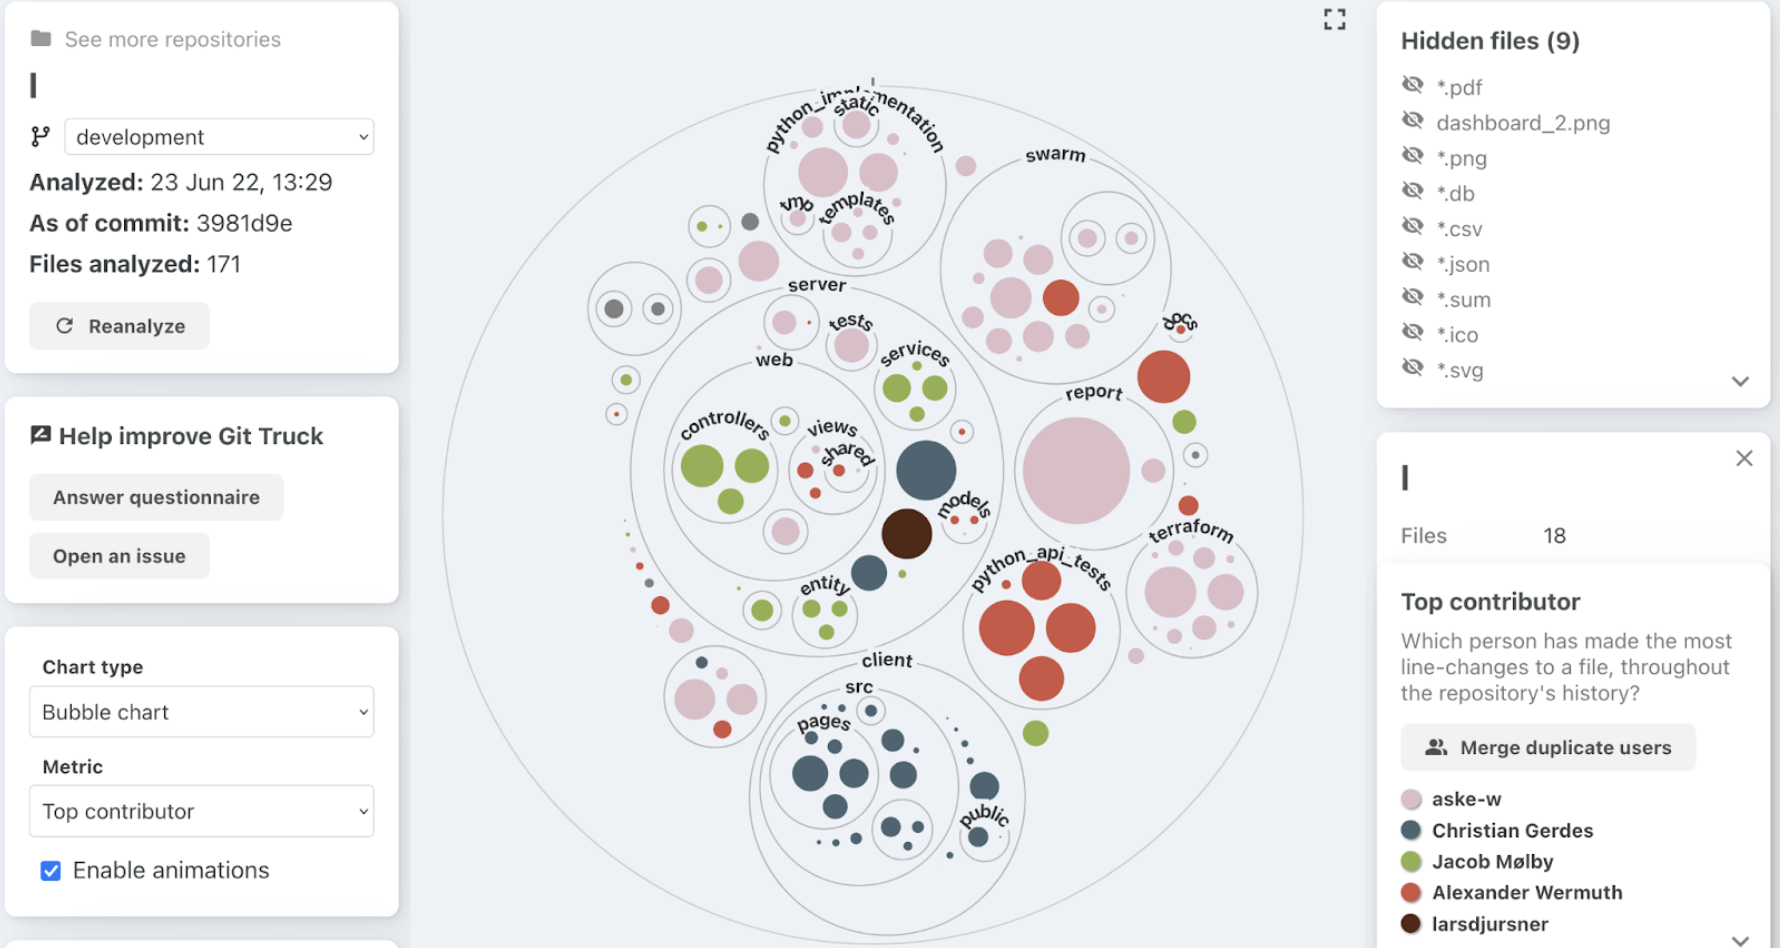
\includegraphics[width=\linewidth]{img/aske_team.png}
    \caption{A system in which students collaborate}
    \label{fig:tid_11}
    \end{figure}




\newpage
\subsection{Visualize Structural Properties to Estimate Software Architecture}

In an introductory web development course we saw two extreme ways of organizing the code structure for implementing the same system with the help of React.js:

\begin{enumerate}
    \item One big CSS file and many JS files as can be seen in Figure \ref{fig:tid_11} where the yellow files are JS and the violet file is the single CSS in the system.

    \begin{figure}[h!]
    \centering
    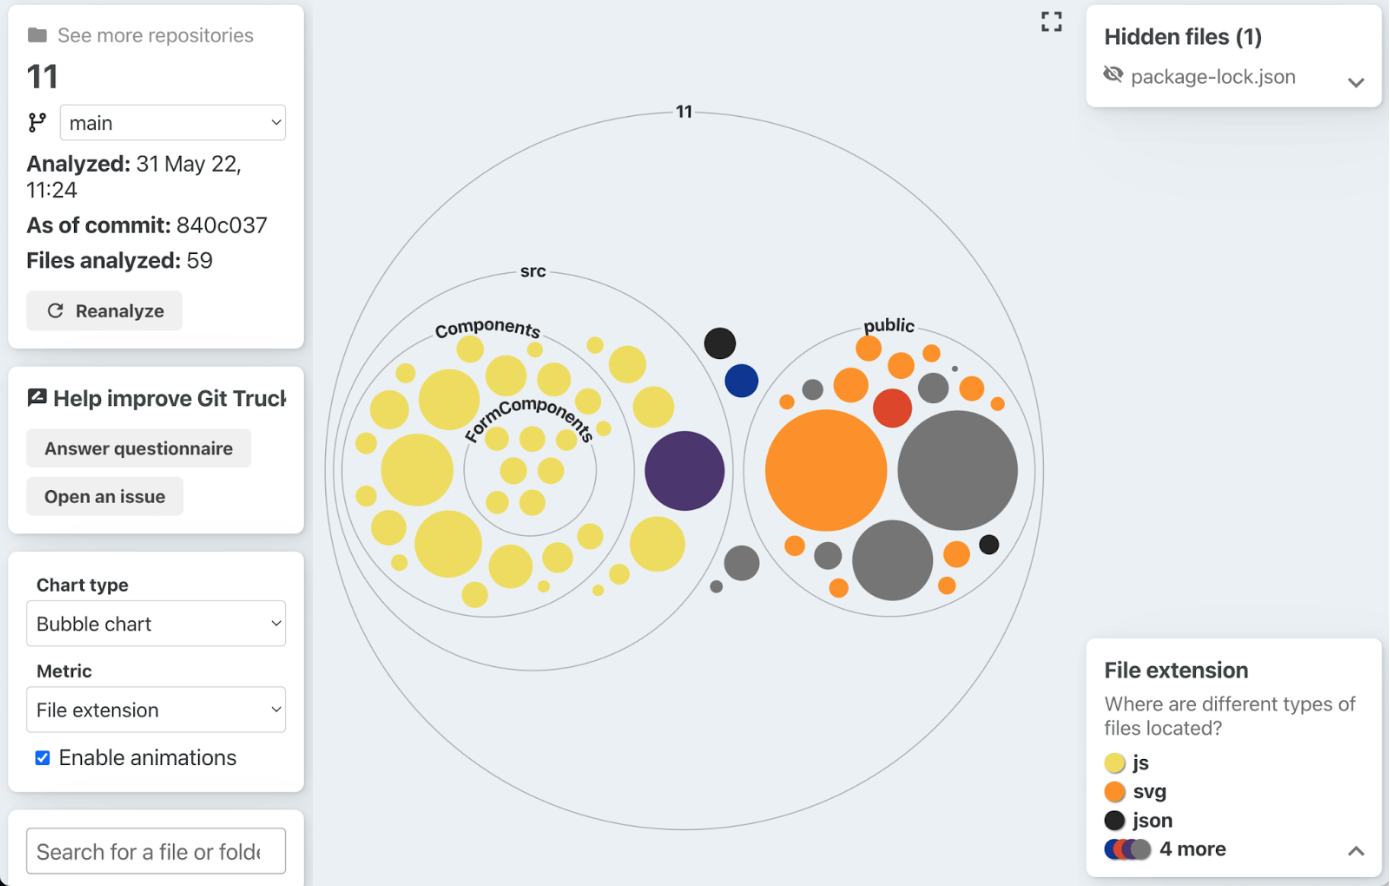
\includegraphics[width=0.8\linewidth]{img/tid_11_wide.png}
    \caption{A system in which the students created a single CSS file}
    \label{fig:tid_11}
    \end{figure}


    \item A CSS file near each JS file as in Figure \ref{fig:tid_10} in which JS files are colored in yellow and CSS files are colored in violet. One can see that the CSS files are distributed through the system.

    \begin{figure}[h]
    \centering
    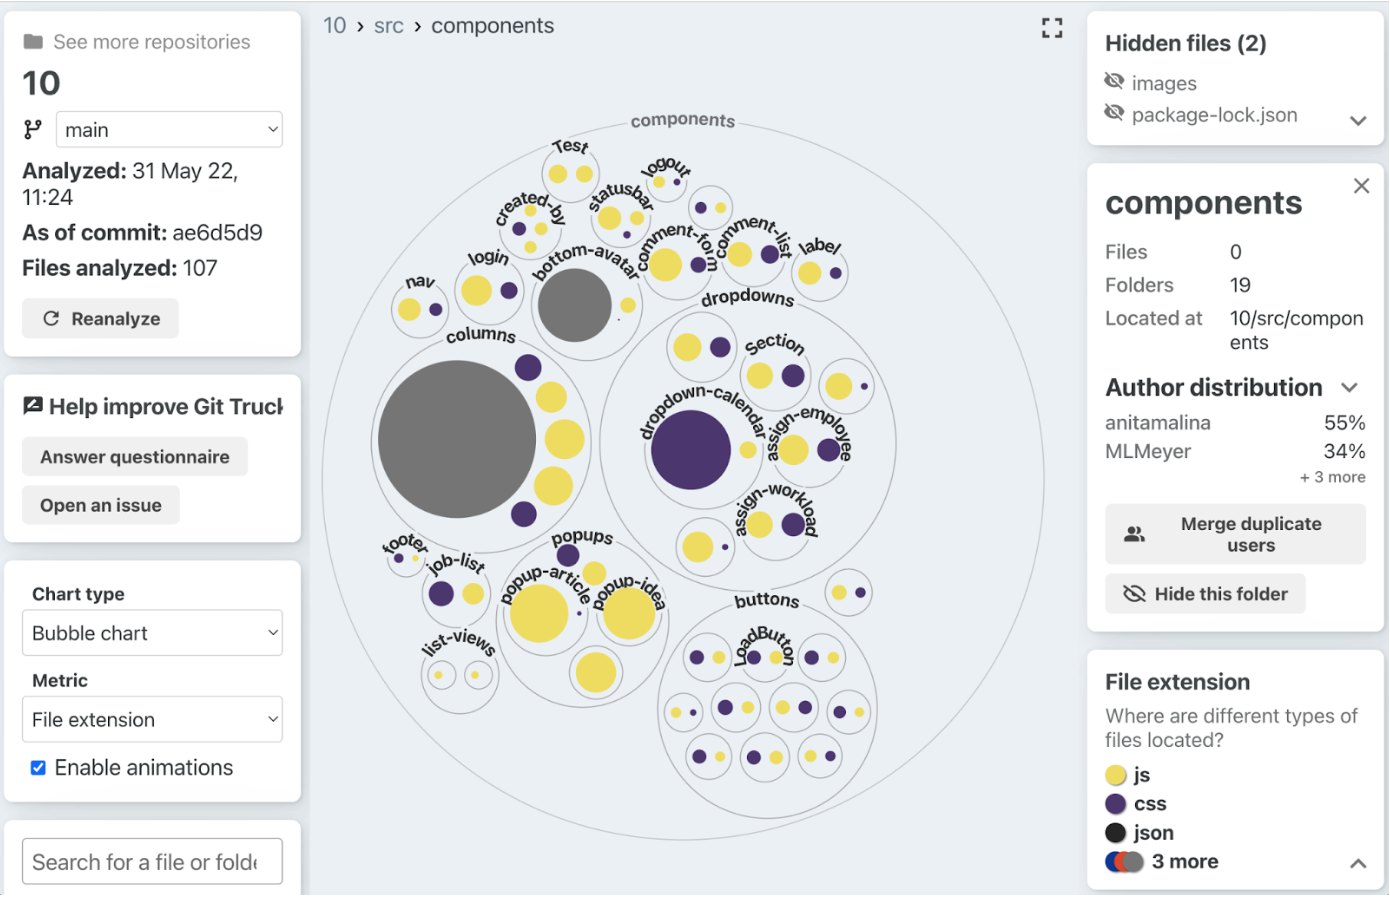
\includegraphics[width=0.8\linewidth]{img/tid_10_wide.png}
    \caption{A system in which the students associated a CSS with a JS file}
    \label{fig:tid_10}
    \end{figure}


\end{enumerate}

Sure, besides the two extremes the teaching team has discovered also many in-between systems. Seeing the diversity of approaches, made the teaching team realize that it would be imperative to discuss file organization in the future iterations of the course. 

\subsection*{Opportunities for Educators}

\begin{itemize}

    \item Can use such project visualizations to better understand the different structures of their student’s projects 

\end{itemize}



\newpage
\subsection{Visualize Change Frequencies to Understand System Behavior Distribution}


The parts of the system that are changed the most are most likely the most “architecturally relevant” parts of the system. An evaluator, would get an impression of which are the most relevant parts of a system by looking at such a view. He could direct their examination towards those parts.

\paragraph{Git Truck (group of four project)}
Figure \ref{fig:truck}} higlights the most changed parts of the git-truck system itself -- which is also a stdent project. The most activity is in the “components” and “analyzer” each of which has one dominant file: 
analyze.server.ts - for the git analysis
chart.ts - for the visualization component. 
However, the effort is quite evenly distributed across the system. 

    \begin{figure}[h]
    \centering
    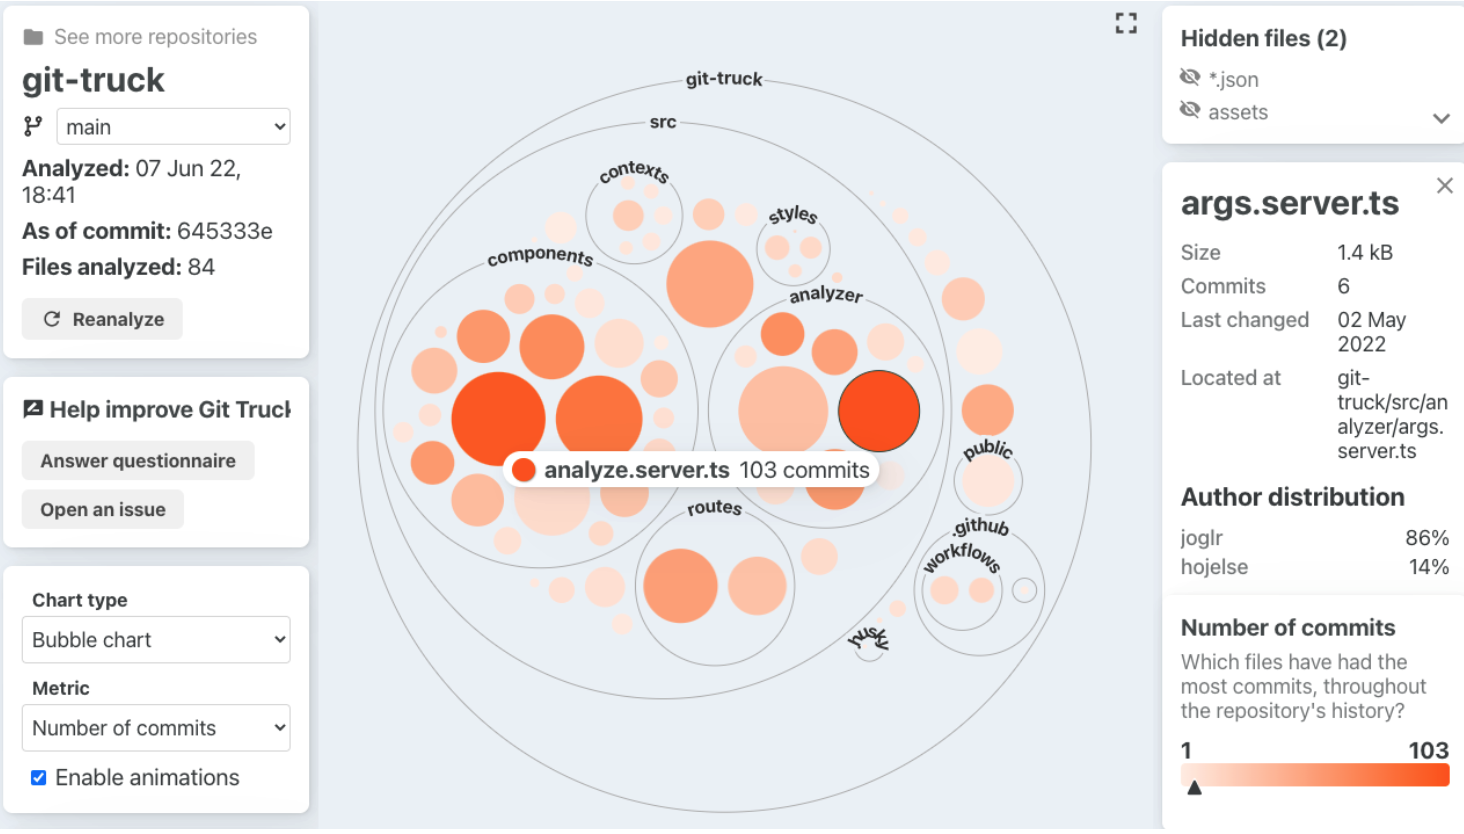
\includegraphics[width=0.9\linewidth]{img/git-truck.png}
    \caption{Git Truck - a system with effort equally distributed across the system}
    \label{fig:truck}
    \end{figure}

\paragraph{Maths Camp - (group of two project; continued by two others in the next year)}

Figure \ref{fig:mathscamp} shows the commit count in Maths Camp -- a system for adaptive maths practice. In the system the commits effort has been disproportionately directed towards a singular JS file. After a closer inspection we learned that the file was very badly designed. 

    \begin{figure}[h!]
    \centering
    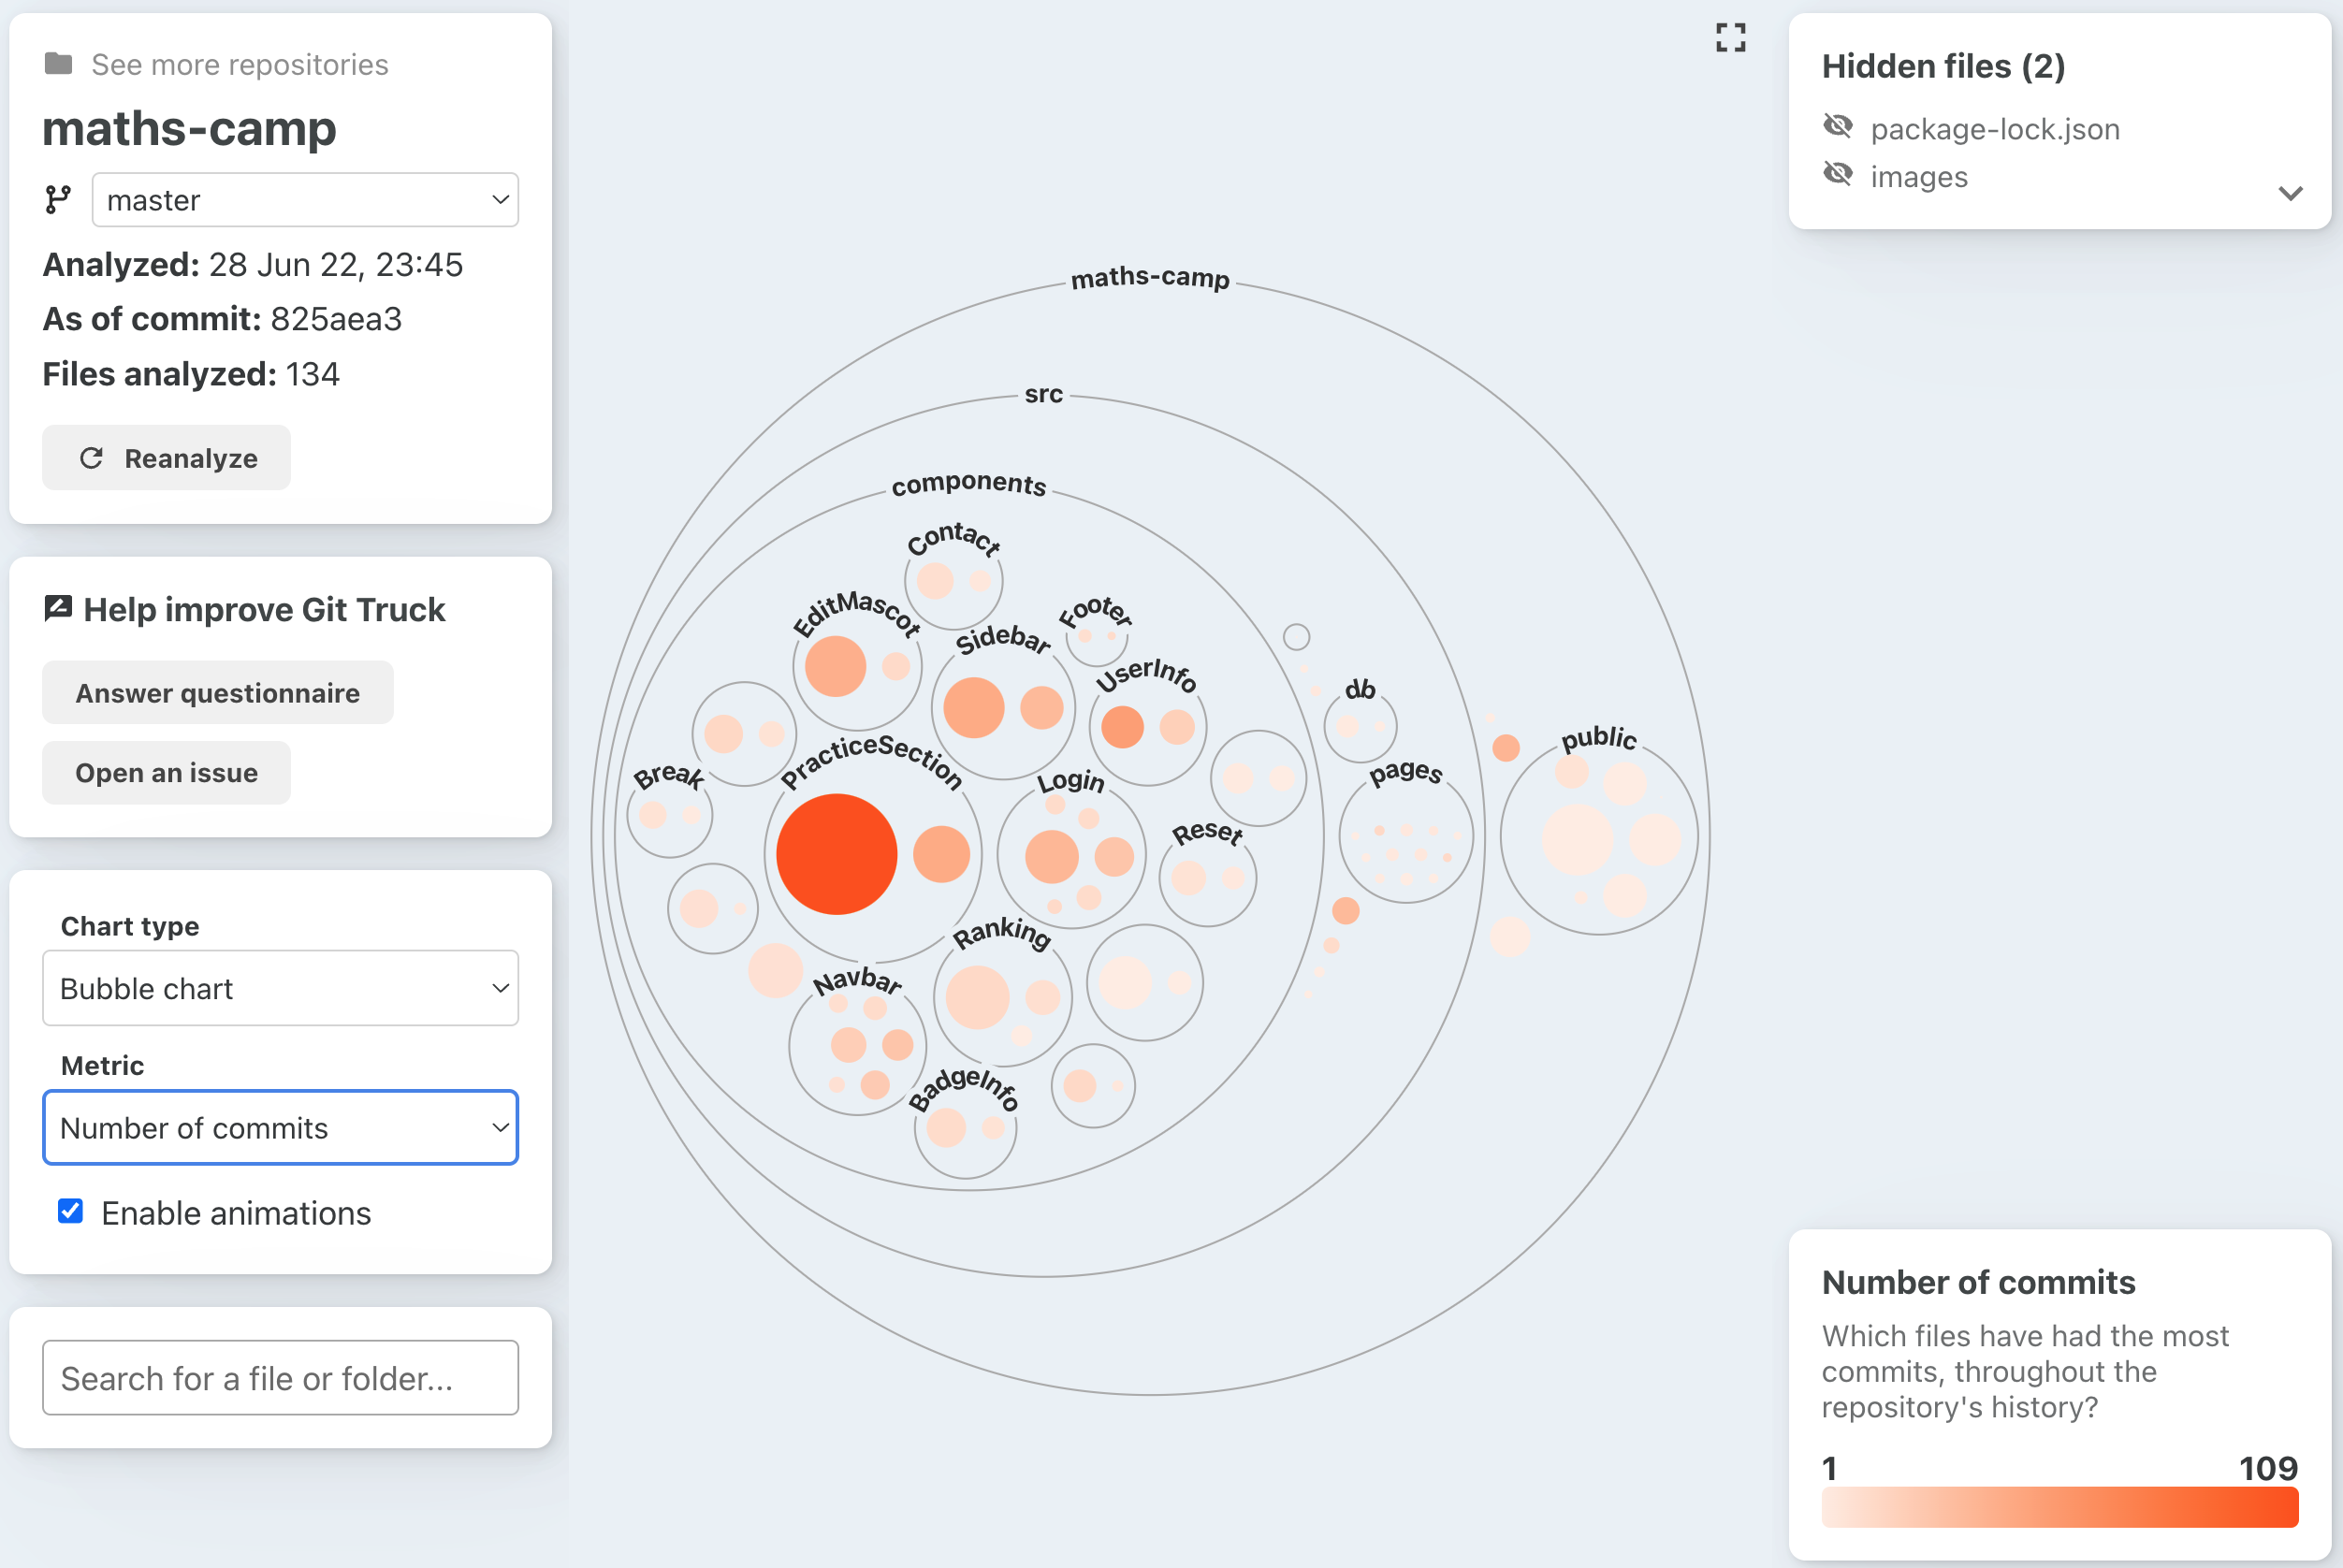
\includegraphics[width=0.9\linewidth]{img/maths-camp.png}
    \caption{Maths Camp - a system where most effort for change goes into a single file}
    \label{fig:mathscamp}
    \end{figure}


However, because the evaluation was done before Git Truck was created, and under time pressure, we browsed the code but did not realize the magnitude of disgrace that this particular component represented: not only large, and with a lot of commits, but was an example of very bad design. With the help of a tool like Git Truck it can be instantly visible. 
% (AD: this could have been probably detected by SonarCloud or similar; Indeed, installing sonar cloud and associated plugins might be a complementary tool for the educator)




\section{Discussion}

\subsection{Threats to Validity}

\subsection{LOC related metrics might be misleading}
Author effort is computed based on the number of lines of code added and removed. However, generated files can be misleading if one relies too much on the effort estimation. 

Current approach, being visual, allows the person inspecting a repository to quickly detect files that are not manually written but rather generated. 

Possible future research direcotin would be: automatically detecting artefacts that are humanly-writte, vs generated. Heuristics based? Language independent?

\subsection{Why not use the visualizations from GitHub?}
For some things GH might suffice. However, not for the ones that rely on “locality” of the various system parts. 

\subsection{Some things can be automatically detected. Why visualize them?}
Some things you can’t think upfront. This is where visualization is needed.
Some things are spatial, and would be hard to present in any other way but visually: e.g. zones of responsibility (UP1). 

\subsection{What is special about git-truck?}
The tool is designed to be as easy to use as possible. However, there is nothing very special about visualizations implemented in git-truck. This is why the patterns presented here should be applicable with other similar tools.

\subsection{What if students work in groups?}
Sometimes the driver in a pair-programming session is not the one to type… GH has co-author annotations. That are supported. 


\subsection{What’s special about educators?}
A tool like this would also serve quite well as a discussion starter in an interview. When a candidate sends a code-base for review, the employer could quickly fire up git-truck and look at the system, to be able to choose some discussion starters. And could represent a vector into further investigating the source code. 



\bibliographystyle{IEEEtran}
\bibliography{bibliography}

\end{document}
